\chapter{Auswertung der Messdaten und Diskussion}

\section{Photolumineszenz (PL)}~\label{sec:PL}
Die gemessene Photolumineszenz der Probe, bei einer Temperatur
von $\pm \SI{4}{\kelvin}$, ist in Abbildung~\ref{fig:photo} zu sehen.
\begin{figure}
    \centering
    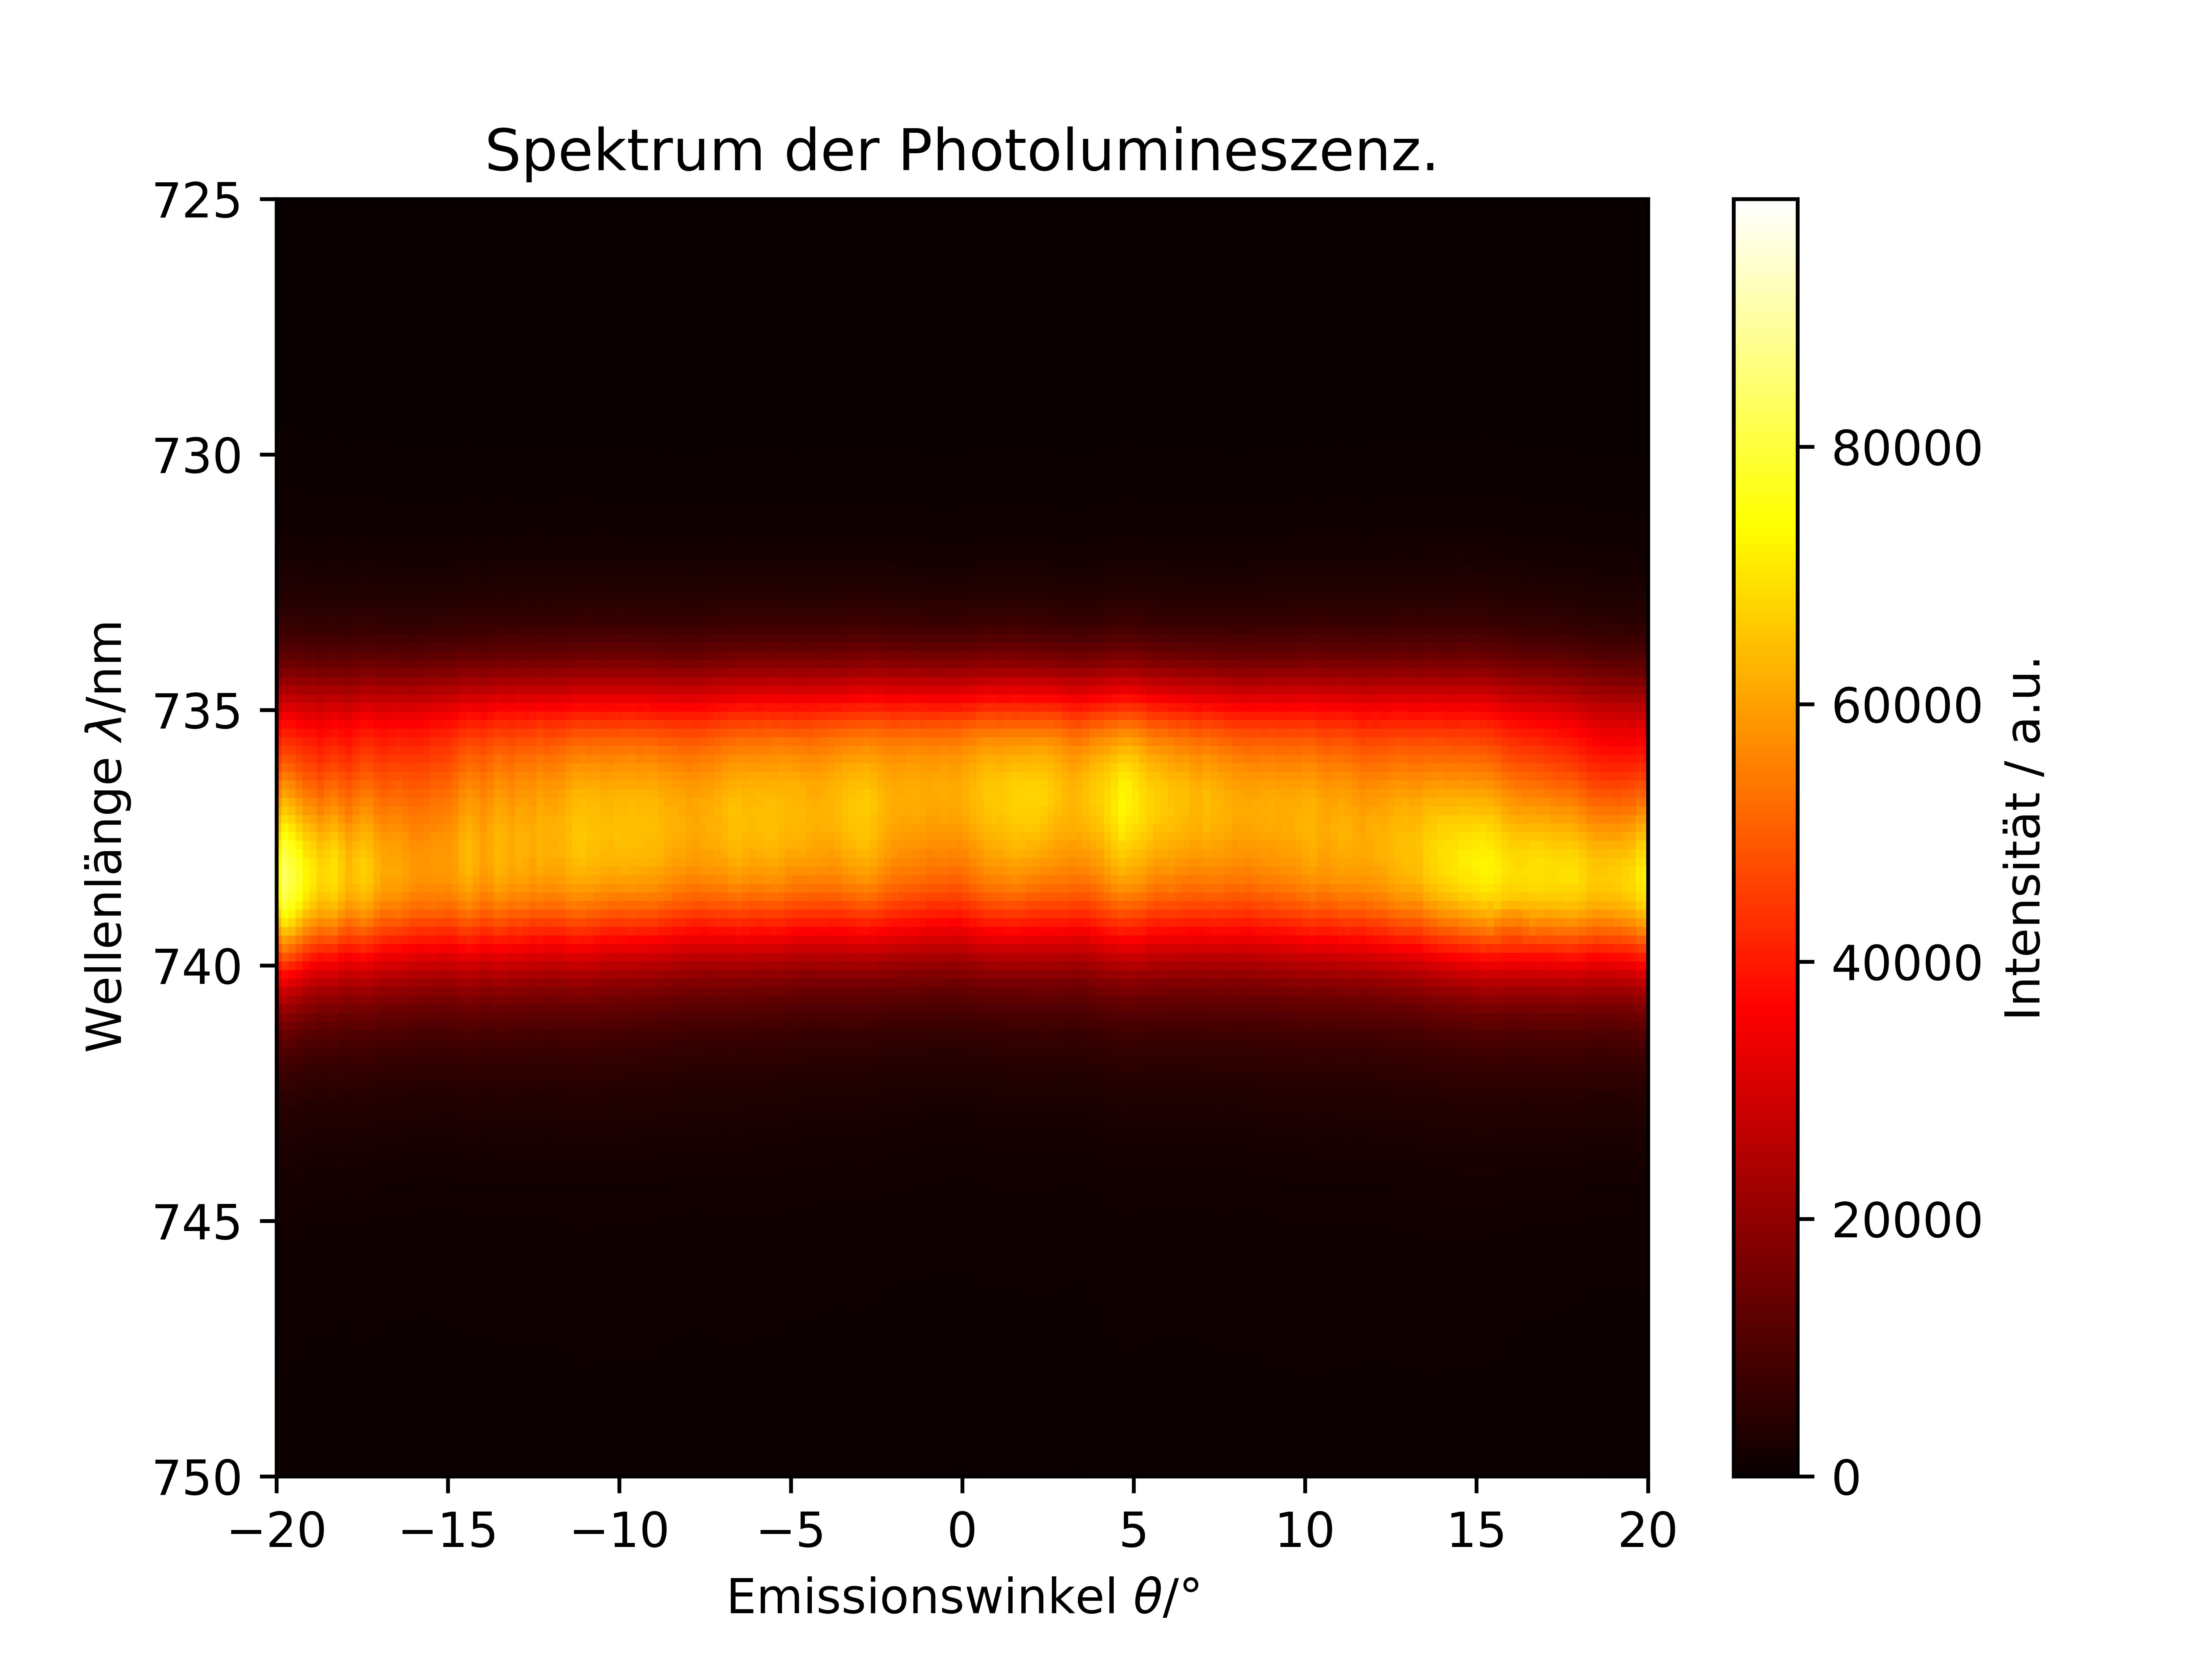
\includegraphics[scale=0.75]{./Plots/colormap__intensity_photolumineszenz_022818A 250nm 4K 2020-07-14.png}
    \caption{Gemessene PL bei einer Temperatur von $\SI{4}{\kelvin}$. Das Maximus ist bei $\SI{738}{\nano\meter}$. }
    \label{fig:photo}
\end{figure}
\FloatBarrier

Das Maximum der PL liegt bei $\SI{738}{\nano\meter}$ was einer Energie $\SI{1,68}{\eV}$ entspricht.
Der Winkelbereich wird bei dieser Messung und allen weiteren Messungen auf $ \theta = \pm \SI{20}{\degree}$ eingeschränkt um 
störende Randeffekte zu vermeiden. 
Die Probe besitzt auf der Oberfläche ein Goldgitter mit einem Gitterabstand 
von $a =\SI{250}{\nano\meter}$ (vgl. Abbildung~\ref{fig:probe}).